\chapter{Program SoundAnalyzer}
\label{kap:programsoundanalyzer}

\section{Koncepce programu}

\emph{SoundAnalyzer} je grafická aplikace pro sledování signálu a jeho kmitočtové charakteristiky v reálném čase. Vytvořil jsem ji pro demonstrování, ale hlavně vyzkoušení pararelizovaného \emph{Goertzelova algoritmu}. Umí zobrazovat vstup z mikrofonu, výstup počítače (monitor výstupu) a také přehrávat zvukový soubor (formát \emph{wav}), nebo získaná data jako zvukový soubor uložit. Umí také provést jednorázový výpočet spektra ze souboru \emph{matlabu} a uložit jej též ve formátu \emph{matlabu}. Má velké možnosti konfigurace pro každý funkční blok (recorder, Goertzelův algoritmus, obecná nastavení).
Ačkoli je v této práci poskytnuta verze pouze pro linux, je program po úpravách multiplatformní.

\section{Použité knihovny}

Grafické uživatelské rozhraní je napsáno v jazyce \emph{QML} a knihovně \emph{Qt}. Tím je dosažena určitá multiplatformnost. Další důvod pro zvolení knihovny \emph{Qt} jsou mé zkušenosti s touto knihovnou a licenční politika.


Pro přehrávání a záznam zvuku ze zařízení je použita knihovna \emph{OpenAL}. Odkazy na funkce z ní jsou výhradně v bloku \emph{recorder}.


Pro zobrazení signálu je použita knihovna \emph{OpenGL}. Její funkční volání je použito výhradně v bloku \emph{barGraphRenderer}.

Vlastní výpočet využívá knihovnu \emph{OpenCL}, které je jako jediná proprietární, ale pro program šířený v rámci \emph{GNU GPLv2} je možné je použít. Jediné použití
\emph{OpenCL} funkcí je v bloku \emph{OpenCLGoertzel}.

Všechny bloku programu jsou pak napsány a pospojovány standardní knihovnou jazyka \emph{C++}. Funkce jazyka \emph{C} nejsou nikde v programu použity.

Více o použitých knihovnách najdete v kapitole \ref{kap:libraries}.

\section{Blokové schéma}
\label{sec:sablockscheme}

Zaměřme se nyní na obrázek \ref{obr:blockscheme}. Vidíme na něm blokové schéma programu \emph{Sound Analyzer}. Nyní proberu jednotlivé části podrobněji.

\begin{figure}
  \begin{center}
    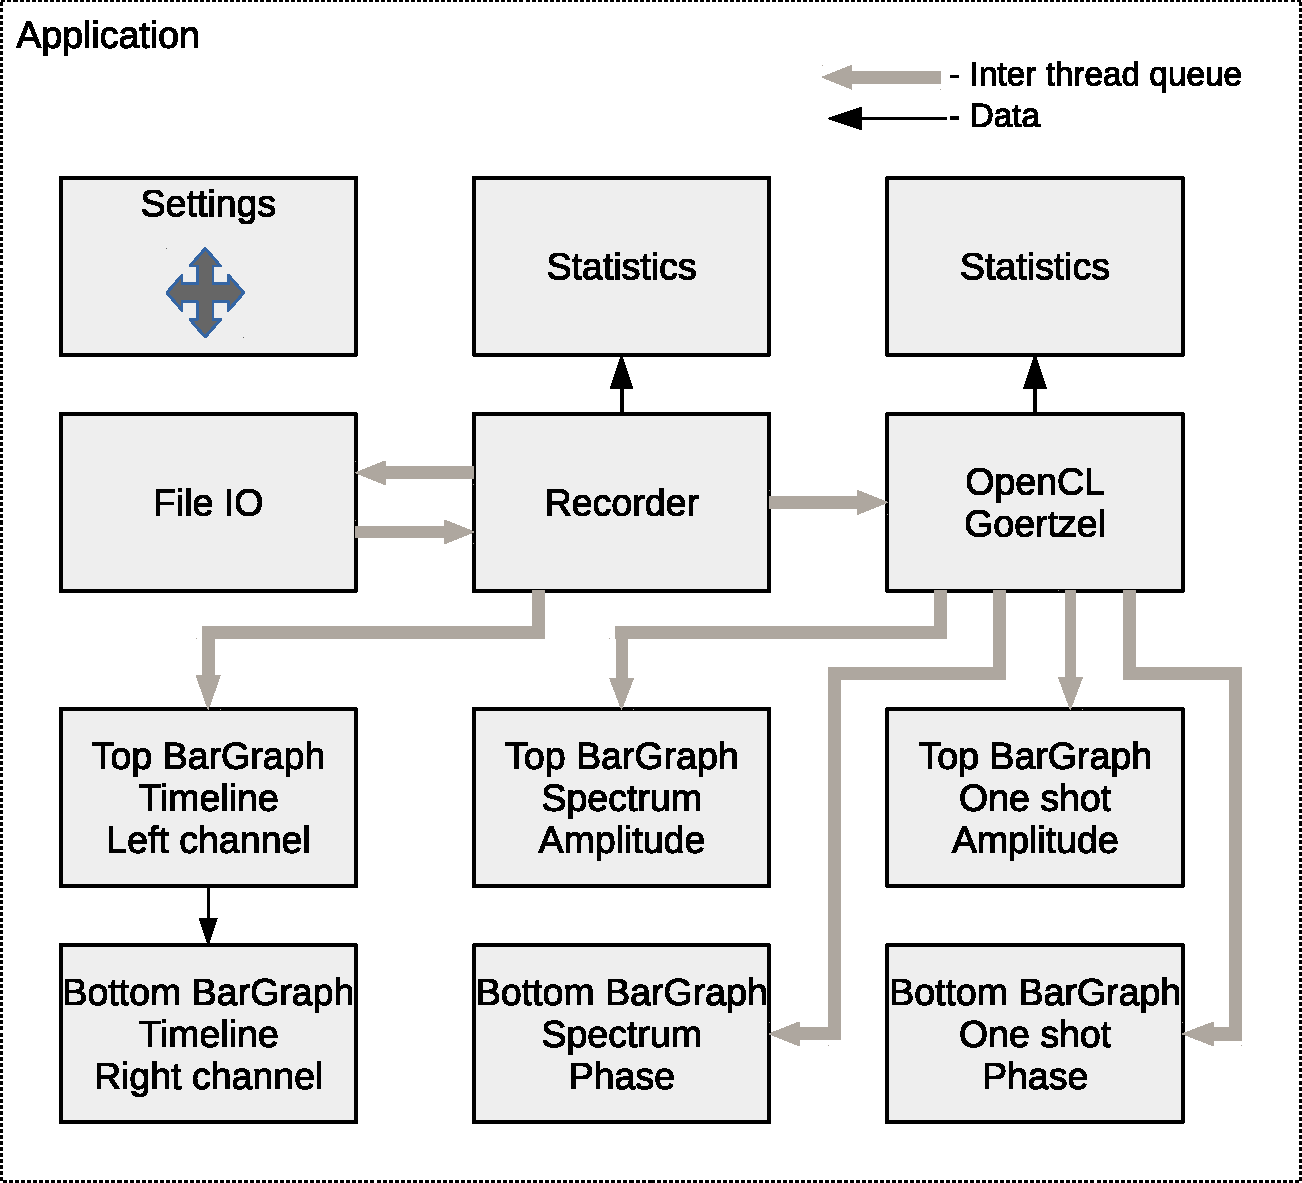
\includegraphics[scale=.7]{obr/SoundAnalyzeBlock}
  \end{center}
  \caption{Blokové schéma programu Sound Analyzer}
  \label{obr:blockscheme}
\end{figure}

\subsection{Inter thread queue}

Aplikace jako tato, která funguje jako přehrávač, záznamník, kreslí do okna
grafy, musí být nutně vícevláknová. Už jen proto, že závisí na spoustě
hardwaru a služeb současně a synchronizace mezi nimi je téměř nemožná.
Procesor totiž střídá vlákna po cca 10ms a pokud by se něco zdrželo ve
vymezeném čase pro hlavní vlákno, docházelo by zcela jistě k trhání a zpomalení
celé aplikace. Tato aplikace má tedy několik téměř samostatných funkcí, každá běžící ve svém vlákně. Problém souběhu řeší tato \emph{mezivláknová fronta}.

Blok \emph{mezivláknová fronta} tedy realizuje frontu opatřenou zámky. Současně poskytuje
zásobu segmentů, které může první vlákno naalokovat, zapsat do nich data a~zařadit do fronty. Druhé vlákno pak segment vyjme z fronty a vrátí. První vlákno nad to ještě může označit segment za poslední a když je přečten, další přečtené segmenty jsou již vždy \emph{nullptr}. Pro účely ladění se kontroluje, zda segment zařazený do fronty a vrácený segment, byly vydány touto frontou. Typická velikost zásoby segmentů je spočítána na cca 1 sekundu vzorků, minimálně však na 10 segmentů.

\subsection{\emph{OpenCL} Goertzel}

\emph{OpenCLGoertzel} je stěžejní komponenta celé aplikace. Vychází ze vztahu \ref{vztah:maticovygoertzelfinal}. Než ale začne samotný výpočet, je třeba spočítat matice $A$ a $D$. Matice $A$ je jednoduchá. Ale i zde lze provést dvě optimalizace. Protože budeme počítat s typem \emph{float -- 32 bitů}, lze očekávat možné nepřesnosti  dané malým počtem bitů. Jedno řešení je tedy jasné -- počítat konstanty v datovém typu \emph{double -- 64 bitů} a převést jen před vlastním zapsáním do grafické karty. Další operace jsou výpočty matice $A^k$, kde se na $k$ díváme jako
na binární číslo.

\begin{myequation}
\begin{aligned}
\label{vztah:rozkladak}
k = \dots k_3 . 2^3 + k_2 . 2^2 + k_1 . 2^1 + k_0 . 2^0 \\
A^k = \dots k_3((AA)(AA))((AA)(AA))  k_2(AA)(AA)  k_1 AA  k_0 A
\end{aligned}
\end{myequation}

tak počítám násobení matice nejvýše 6krát a nikoli 15krát jako kdybych počítal
prostým cyklem. Pokud mám různé mocniny $A$, snadno určím matici $D$.

Pokud bychom řekli, že sčítání mezivýsledků a počítání jednoho mezivýsledku dle vzorce \ref{vztah:maticovygoertzelfinal} trvá stejně dlouho, (jsou tam stejné matematické operace) dojdeme k~závěru, že optimální by bylo rozdělit výpočet série $N$ vzorků na
$N_M$.$N_L$ operací, kde $N_M$ a $N_L$ jsou stejné (přibližně odmocniny z $N$). Takto také tato komponenta počítá kolik cyklů ($L$) a kolik jader ($M$) bude použito pro výpočet. Já jsem v programu \emph{Sound Analyzer} ze začátku skutečně proměnné $L$ a a $M$ zavedl. Nyní se to již zdá být zbytečné, nicméně je to v programu stále, protože se ukázalo, že předpoklad ze začátku tohoto odstavce není úplně splněn a možná bude lepší jiný  algoritmus pro stanovení $L$ a $M$. Protože je možné doplnit řadu vzorků nulami, aniž by se ovlivnil výpočet, udělám to a zajistím si tak, že programy jader budou jednodušší, protože všechna jádra budou počítat stejný počet cyklů. Nakonec ani není třeba řešit, pokud by odmocnina z $N$ bylo iracionální číslo, prostě proměnné $L$ a $M$ zaokrouhlím nahoru. Ještě dodejme, že nuly se musí přidat před vzorky signálu, nikoli za něj.


Tato komponenta umí počítat nejen ze vzorků čerstvě přišlých z \emph{mezivláknové fronty}, ale i několika až $16386$ vzorků předchozích. Je tak možno získat větší přesnost, ale za cenu toho, že počítáme z delšího intervalu a výsledky tak nemusejí odpovídat okamžité realitě.


Na závěr sekce se zmíním o velikosti vektorů, se kterými lze počítat v knihovně \emph{OpenCL}. V dokumentaci \emph{OpenCL} je uvedena maximální velikost $16$ s tím, že je implementačně závislá a program si musí zjistit skutečnou velikost vektoru.
V případě mého grafického čipu \emph{AMD 7850} je to hodnota $8$. Ovšem já potřebuji složky vektoru sečíst a funkce, která to provádí, má podle dokumentace další omezení -- na velikost $4$. Nakonec tedy počítám s velikostí $4$. \emph{OpenCL} neumožňuje maticové operace.

Vlastní \emph{jádro}\ref{sec:kernel} je velmi jednoduché:

\begin{Verbatim} 

__kernel void main(
    __constant float*   streams,   //vstupní segment signálu
    __constant float*   D1,        //horní řádek matice D
    __constant float*   D2,        //dolní řádek matice D
    unsigned int        Channels,  //počet kanálů
    unsigned int        K,         //délka vektoru OpenCL, konstanta 4
    unsigned int        L,         //počet cyklů, respektive délka vektoru
                                   // se kterým pracujeme / 4
    unsigned int        M,         //počet jader spuštěných nad algoritmem
                                   // pro jeden kmitočet, jeden kanál		                               
    unsigned int        Length,    //délka segmentu
    __global float2*    outStreams //výtupní vektor
)
{
    unsigned int indexFrequency = get_global_id(0);
    unsigned int indexChannel = get_global_id(1);
    unsigned int indexItem = get_global_id(2);
    unsigned int i;
    float2 acc={0.0,0.0};
    __constant float4* data = (__constant float4*)&streams[indexChannel 
    		* Length + indexItem * L * K];
    __constant float4* mxD1 = (__constant float4*)&D1[indexFrequency 
    		* L * K];
    __constant float4* mxD2 = (__constant float4*)&D2[indexFrequency 
    		* L * K];
    for(i=0;i<L;i++)
    {
        acc.x = acc.x + dot(data[i] , mxD1[i]);
        acc.y = acc.y + dot(data[i] , mxD2[i]);
    } 
    outStreams[indexFrequency * Channels * M + indexChannel * M 
    		+ indexItem] = acc;
}
\end{Verbatim}

Funkci, jež má modifikátor \emph{\_\_kernel} \ref{sec:kernel} umíme jako jedinou spustit z hlavního programu a říkáme jí \emph{jádro}. Naše funkce má 9 parametrů, které mají před svými jmény modifikátory specifikující, ve které paměťové třídě se proměnná nachází. Více o těchto paměťových třídách najdete v kapitole \ref{kap:opencl}. Jak je vidět, program pouze realizuje cyklus:

\begin{myequation}
\begin{aligned}
\label{vztah:mojevariacestavw0_1}
outStreams[i_c][n] = \\
( \sum_{n=0}^{L-1} streams[i_c][n] . D_1[i_f][n] , \sum_{n=0}^{L-1} streams[i_c][n] . D_2[i_f][n] ),
\end{aligned}
\end{myequation}

kde $stream$ je blok vstupního signálu a $D_1[kmitočet],D_2[kmitočet]$ jsou přepočítané řádky matice $D$. Index kmitočtu je pak $i_f$ a index kanálu je $i_c$.


\subsection{Recorder}

\emph{Recorder} plní mezivláknovou frontu segmenty pro výpočet. Načítá je ze vstupního zařízení. Implicitní je určitě mikrofon, dále je možnost vybrat monitor výstupu, tedy provádět výpočet spektra nad signálem poskytovaným jinou aplikací. Volitelně může navíc ještě segmenty zkopírovat k zapsání do souboru komponentou popsanou níže.

Druhý režim \emph{recorderu} je přehrávání. Segmenty pořízené komponentou \emph{FileIO} jsou přehrány na standardním výstupu a zkopírovány do fronty pro výpočet spektra. Tím že jsou do této fronty kopírovány právě v okamžiku po jejich přehrání, je zajištěno časování.

Pokud je zvolen monitor standardního výstupu, nebo monitor HDMI výstupu, je signál zkreslen. Domnívám se, že je to ochrana proti kopírování. Záznam zvuku z~těchto monitorů totiž není zatížen ani minimálním šumem.

\subsection{File IO}

Souborové operace v programu \emph{Sound Analyzer} jsou načítání zvukového souboru ve formátu \emph{wav} do \emph{mezivláknové fronty} a samozřejmě i směrem z \emph{mezivláknové fronty} do souboru. V případě, že služby souborového systému jsou pomalejší než přísun segmentů,
jsou ve výsledném \emph{wav} souboru nespojitosti v tom smyslu, že je soubor je validní, dá se přehrát, ale jeho obsah je nespojitý.  Je také vypisováno hlášení na konzoli.
V případě, že souborový systém není schopen dodat dostatek dat pro přehrávání, mezivláknová fronta je prázdná a přehrávání je přerušované. I zde je vypisováno varovné hlášení na konzoli.


\subsection{Stats}

Komponenta statistiky je velmi jednoduchá. Má jen frontu hodnot a vždy zná jejich součet. Umí tak poskytnout kmitočet obnovování, vzorkovací kmitočet a  průměrný čas výpočtu spektra. Jednou za 0,5s vrací příznak, že komponenta, která statistiku vlastní, může zobrazit své data v uživatelském prostředí.

\subsection{Settings}


Nastavení je malá množina párů hodnota-klíč, sloužící k uchování nastavení. Její výhoda je přístup jak z \emph{C++}, tak z jazyka \emph{QML}. Po skončení aplikace se její obsah uloží do souboru a po startu je načten zpět.

\subsection{Application}

Aplikace všechny výše uvedené komponenty spojuje. Komponenty v \emph{Sound Analyzeru} jsou striktně odděleny a pokud spolu potřebují komunikovat nebo něco zobrazit, využívají funkce komponenty aplikace. Aplikace je jediná komponenta svázaná s grafickou knihovnou \emph{Qt}. Je ještě jedna funkce, kterou aplikace má. Při zapnutí nastaví všechny komponenty podle nastavení v komponentě settings a při změně pohledu mění propojení mezivláknových front.

\section{Licence}

Všechny použité knihovny jsou šířeny, nebo podporují \emph{GNU licenci}, takže i má práce musí být šířena pod licencí \emph{GNU GPLv2}.